\documentclass[12pt]{article}

\usepackage{xspace}
\usepackage{lineno}
\usepackage{setspace}
\usepackage{graphicx}
\usepackage{subfigure}
\usepackage{float}
\usepackage{color}
\usepackage{caption}
\usepackage[margin=1in]{geometry}
\usepackage{natbib}
\usepackage{amsmath}


\begin{document}
\doublespacing
\linenumbers

\newcommand{\kluyveri}{\textit{L. kluyveri}\xspace}
\newcommand{\dubl}{\textit{C. dubliniensis}\xspace}
\newcommand{\gossypii}{\textit{E. gossypii}\xspace}
\newcommand{\ROC}{ROC SEMPPR\xspace}
\newcommand{\GC}{GC content\xspace}

\noindent RH: LANDERER ET AL.--- Intragenomic variation in codon usage
% put in your own RH (running head)
% for POVs the RH is always POINT OF VIEW
\bigskip
\medskip
\begin{center}

% Insert your title:
\noindent{\Large \bf Differences in Codon Usage Bias between genomic regions in the yeast \textit{Lachancea kluyveri}.}
\bigskip

% We don't use a special title page; the author information is entered
% like any other text.

% FOOTNOTES: We don't allow them in the manuscript, except in
% tables. Don't include any footnotes in the text.


\noindent{C\textsc{EDRIC} ~{L\textsc{ANDERER}}$^{1,2,*}$,
R\textsc{USSELL} {Z\textsc{ARETZKI}}$^{3}$,
\textsc{AND}
M\textsc{ICHAEL} A.~{G\textsc{ILCHRIST}}$^{1,2}$}

\end{center}

\vfill

{\small
\noindent$^{1}$Department of Ecology \& Evolutionary Biology, University of Tennessee, Knoxville, TN 37996-1610\\
\noindent$^{2}$National Institute for Mathematical and Biological Synthesis, Knoxville, TN 37996-3410\\
\noindent$^{3}$Department of Business Analytics \& Statistics, Knoxville, TN ~ 37996-0532 \\
\noindent$^{*}$Corresponding author. E-mail:~cedric.landerer@gmail.com
}

\vfill
\centerline{Version dated: \today}
\vfill
\newpage

\begin{abstract}
Codon usage has been used as a measure for adaptation of genes to their genomic environment for decades. 
The introgression of genes from one genomic environment to another may cause well adapted genes to be suddenly less adapted due to their signature of a foreign genomic environment.
The reflection of a foreign genomic environment in transferred genes can result in a large fitness burden for the new host organism.
%However, it is possible to observe the opposite, as genes can be exapted; for example if mutation bias in the donating organism matches selection bias in the receiving organism.
Here we examine the yeast \textit{Lachancea kluyveri} which has experienced a large introgression, replacing the left arm of chromosome C ($\sim 10 \%$ of its genome).
The \kluyveri genome provides an opportunity to study the adaptation of introgressed genes to a novel genomic environment and estimate the fitness cost such a transfer imposes.
The codon usage of the endogenous \kluyveri genome and the exogenous genes were analyzed, using \ROC which allows for the effects of mutation bias and selection bias on codon usage to be separated.
We found substantial differences in codon usage between the endogenous and exogenous genes, and show that these differences can be largely attributed to a shift in mutation bias from A/T ending codons in the endogenous genes to C/G ending codons in the exogenous genes.
Recognizing the two different signatures of mutation and selection bias improved our ability to predict protein synthesis rate by $17 \%$ and allowed us to accurately assess codon preferences.
In addition we utilize the estimates of mutation bias and selection bias gaines using \ROC to determine a potential source lineage, estimate the time since introgression and asses the fitness burden the introgressed genes represent showing the advantage of mechanistic models have when analyzing codon data.
%In order to identify a potential source of the exogenous genes, we estimated mutation and selection bias across 38 yeast lineages. Our initial comparison identified two candidates, \textit{Candida dubliniensis}  and \textit{Eremothecium gossypii}, as potential source linages.
%We excluded \dubl using orthogonal information on synteny.
%We also estimated that the exogenous genes introgressed $6.22\times10^8$ generation ago into the \kluyveri genome.
\end{abstract}
\newpage

\section*{Introduction}
\begin{itemize}
	\item A genes codon usage reflects the genomic environment it has evolved in.
	\begin{itemize}
		\item Mutation, selection, and drift are fundamental forces shaping the genomic environment.
		\item The strength and efficacy of selection on codon usage is generally positively correlated with gene expression
		\item On the other hand, the efficacy of mutation on codon usage is generally negatively correlated with gene expression.
		\item Together, mutation driven bias - or mutation bias - and selection driven bias scaled by gene expression - or selection bias - shape codon usage in a genome; allowing us to describe the genomic environment in which genes evolve with respect to these terms.
		\item Estimating the influence of mutation bias and selection bias on a gene improves our understanding of its evolution; giving us the ability to describe its history and making predictions about its future.
	\end{itemize}
	\item Most studies implicitly assume that codon usage of a genome is the product of a single genomic environment.
	\begin{itemize}
		\item This assumption however, can be violated by horizontal gene transfer, introgression, or hybridization.
		\item The transfer of genes to a different genomic environment may cause them to be less adapted to the novel environment, with potentially large fitness consequences if the two genomic environments differ greatly in their selection bias, making such transfers less likely.
		%\item In contrast, similarities in the genomic environment could, under certain circumstances even promote the transfer of genomic material. 
		\item Furthermore, if unaccounted for, introgressed genes may distort parameter estimates describing codon usage and cause us to conclude wrong codon
	\end{itemize}
	\item In this study we analyze the synonymous codon usage in the genome of \kluyveri, the earliest diverging lineage of the Lachancea clade.
	\begin{itemize}
		\item The Lachancea clade diverged from the Saccharomyces lineage prior to the whole genome duplication about 100 Mya ago.
		\item Since diverging from the other Lachancea, \kluyveri has experienced a large introgression of exogenous genes replacing the whole left arm of chromosome C. 
		\item This chromosome arm has a \GC  $\sim 13 \%$ higher than the endogenous \kluyveri genome.
	\end{itemize}
	\item Using \ROC allows us to describe the genomic environment genes have evolved in by separating effects of mutation bias and selection bias, and predict protein synthesis rate.
	\begin{itemize}
		\item We use \ROC to describe two genomic environments reflected in the \kluyveri genome, an endogenous and an exogenous environment.
		\begin{itemize}
			\item We attribute most of the in GC bias to differences in mutation bias.
		\end{itemize}
		\item Recognizing differences in codon usage between endogenous and exogenous genes improves our ability to predict protein synthesis rate. 
	\end{itemize}
	\item In addition to improvements to model fitting, we show the utility of the quantitative estimates from \ROC of mutation bias and selection bias, and protein synthesis rate by:
	\begin{itemize}
		\item Determining a potential source lineage of the introgressed exogenous genes.
		\begin{itemize}
			\item Comparing the estimates of $\Delta M$ and $\Delta \eta$ for the exogenous gene region to 38 yeasts and identified ancestors of \gossypii and \dubl as most likely sources of the introgression.
		\end{itemize}
		\item Estimate the time since introgression and the persistence of the signal of the exogenous environment.
		\item Estimate the selective cost of mismatched codon usage bias at gene and chromosome scale of the introgression.
	\end{itemize}
\end{itemize}

\section*{Results}
	
\begin{itemize}
	\item We compared model fits of \ROC to the full \kluyveri genome, and the separated endogenous and exogenous genes.
	\begin{itemize}
		\item We find that the partitioning of the \kluyveri genome into endogenous and exogenous genes and estimating separate mutation and selection bias parameters is clearly favored ($\Delta AIC \sim 90,000$).
		\item Treating endogenous and exogenous genes as separate sets:
		\begin{itemize}
			\item improves our relative ability to predict protein synthesis rate by $17 \%$ ($\rho = 0.59$ vs. $\rho = 0.69$), (Figure \ref{fig:phi_corr_two_cond}).
			\item avoids inference of incorrect codon preferences  (Figure \ref{fig:csp_comp}). .
		\end{itemize}
	\end{itemize}
	\item Larger differences in mutation bias than selection bias between the historical genomic environment of the endogenous and exogenous genes (Figure \ref{fig:csp_comp}).
	\begin{itemize}
		\item Mutation is biased towards A/T ending codons ($11/19$) in the endogenous genes and strongly biased towards C/G ending codons ($17/19$) in the exogenous genes.
		\item Only two amino acids (A,F) showing complete concordance in mutation bias.
		\item In contrast, we find the same codon preference in endogenous and exogenous genes for nine amino acids. 
		\item We also observe a stronger selection bias towards C/G ending codons reflected in the exogenous genes. 
	\end{itemize}
	\item We inferred potential source lineages by comparing codon usage bias and synteny of yeast lineages to the exogenous region
	\begin{itemize}
		\item 33 out of 38 lineages showed similar selection bias
		\item four lineages showed similarity in mutation bias (\gossypii, \dubl, and \textit{Sphaerulina musiva}, \textit{Yarrowia lipolytica}).
		\item Only \gossypii and \dubl had a strong positive relationship in both mutation bias and selection bias. 
		\item synteny between \gossypii and \dubl and closely related lineages and the exogenous genes left only \gossypii as candidate.
		\begin{itemize}
			\item Synteny with the exogenous region is limited to the Saccharomycetacease group.
		\end{itemize}
	\end{itemize}
	\item We predict the age of the introgression using an exponential model of decay.
	\begin{itemize}
		\item We estimate the age to be about $6\times10^8$ generations.
		\item The signature of the sources genomic environment will decay to one percent of the \kluyveri genomic environment in about $5\times10^9$ more generations.
	\end{itemize}
	\item We estimate the fitness burden of the introgressed region on \kluyveri and compare it to the fitness burden at the time of introgression.
	\begin{itemize}	
		\item assuming constant \gossypii genomic environment and amino acid usage. 
		\item We find that the exogenous genes:
		\begin{itemize}
 			\item were a large fitness burden at the time of introgression (Figure \ref{fig:sne_fitness_burden}).
			\item still represent a large reduction in fitness relative to the replaced expected endogenous genes (Figure \ref{fig:sne_fitness_burden}).
		\end{itemize}
	\end{itemize} 
\end{itemize}

\section*{Discussion}

\begin{itemize}
	\item Following Payen et al. (2009), we partitioned \kluyveri into endogenous and exogenous genes using gene location.
	\item Estimating codon usage parameters using \ROC, we find:
	\begin{itemize}	
 		\item two gene sets show difference in mutation bias and selection bias
		\begin{itemize}
			\item Endogenous genes tend to be generally  biased towards A/T ending codons while exogenous genes are biased towards C/G ending codons.
			\item We observe higher correlation between $\Delta \eta$ than $\Delta M$, nevertheless we find the optimal codon differs between endogenous and exogenous genes in nine out of 19 synonymous codon families. 
			\item Without recognizing the difference in codon preference we would have inferred the preferred codon in the \kluyveri genome wrong for seven amino acids.
			\end{itemize}
		\item We also improve our relative ability to predict protein synthesis rate when separating endogenous and exogenous genes by $17 \%$. 
	\end{itemize}
	\item To identify a potential source lineage for the exogenous genes, we:
	\begin{itemize}
		\item compared of $\Delta M$ and $\Delta \eta$ estimates from the exogenous genes to 38 other yeast lineages.
		\begin{itemize} 
			\item revealing 33 and five yeast lineages showing a positive relationship in selection bias and mutation bias, respectively.
		\end{itemize}
		\item compared synteny of the exogenous region:
		\begin{itemize}
			\item finding consistency only within the Saccharomycetaceae clade.
			\item Most of the eight species with synteny showed similarity in selection bias but not in mutation bias.	
			\item Only \gossypii showed both synteny with the exogenous region and a similar mutation and selection bias.
		\end{itemize}
	\end{itemize}
	\item We estimated the age of the introgression to be on the order of  $6.22\times10^8$ generation using our estimates of $\Delta M$ from the exogenous genes and \gossypii.
	\begin{itemize}
		\item Assuming a constant genomic environment in the \kluyveri and \gossypii genome.
		\item The slower decay of mutation bias relative to selection bias also allowed us to estimate the time until the introgression will have decayed to be about $5.66\times10^9$ generations.
		\begin{itemize}
			\item Differences in selection bias are expected to have decayed earlier.
			\item This is consistent with the observation that HGT is more common between lineages with simlar codon preference, as most methods (CAI, tAI) focus only on selection. As a result, they are insensitive to differences in mutation bias.
		\end{itemize}
	\end{itemize}
	\item Assuming that the current amino acid sequence is representative of the ancestral, we estimate the fitness burden at the time of introgression of the exogenous genes on \kluyveri compared to the endogenous genes with the expected ancestral codon usage.
	\begin{itemize}
		\item As expected, low expression genes have a relatively small impact on fitness, and adapt more slowly to the endogenous environment.
		\item Estimating the impact the exogenous genes had on the fitness of \kluyveri at the time of the introgression revealed that this event was very unlikely to reach fixation.
		\item It is hard to contextualize the probability of this introgression going to fixation as we are not aware of any estimates of the frequency at which such large scale introgressions of genes with very different signatures of mutation and selection bias occur.
		\begin{itemize}
			\item However, e.g. \kluyveri diverged about 85 Mya, with one to eight generations per day, or $10^{10}$ to $10^{11}$ generations ago from the rest of the Lachancea clade. Assuming an effective population size on the order of $10^8$, we are left with $10^{18}$ to $10^{19}$ opportunities for such an event to occur.
		\end{itemize}
		\item We also show that the exogenous genes still represent a large decrease a fitness relative to the hypothesized ancestral endogenous genes.
	\end{itemize}	
	\item In conclusion, we show the usefulness of the separation of mutation bias and selection bias in this study of codon usage and we illustrate how \ROC can be used for more sophisticated hypothesis testing in the future.
	\begin{itemize}
		\item We highlight potential pitfalls when estimating codon preference, as estimates can be biased by the signature of a second, historical genomic environment.
		\item In addition, we show how estimates of selection relative to drift can be obtained from codon data and used to infer the fitness cost of introgressed genes.
	\end{itemize}
\end{itemize}

\clearpage

\section*{Figures}

\begin{figure}[h]
    \centering
    \begin{subfigure}
        \centering
        \includegraphics[width=.45\textwidth]{img/csp_corr_dm.pdf}
    \end{subfigure}
    \begin{subfigure}
        \centering
        \includegraphics[width=.45\textwidth]{img/csp_corr_deta.pdf}
    \end{subfigure}
    \caption{Parameters are relative to mean}
    \label{fig:csp_comp}
\end{figure}

\begin{figure}[h]
    \centering
    \begin{subfigure}
        \centering
        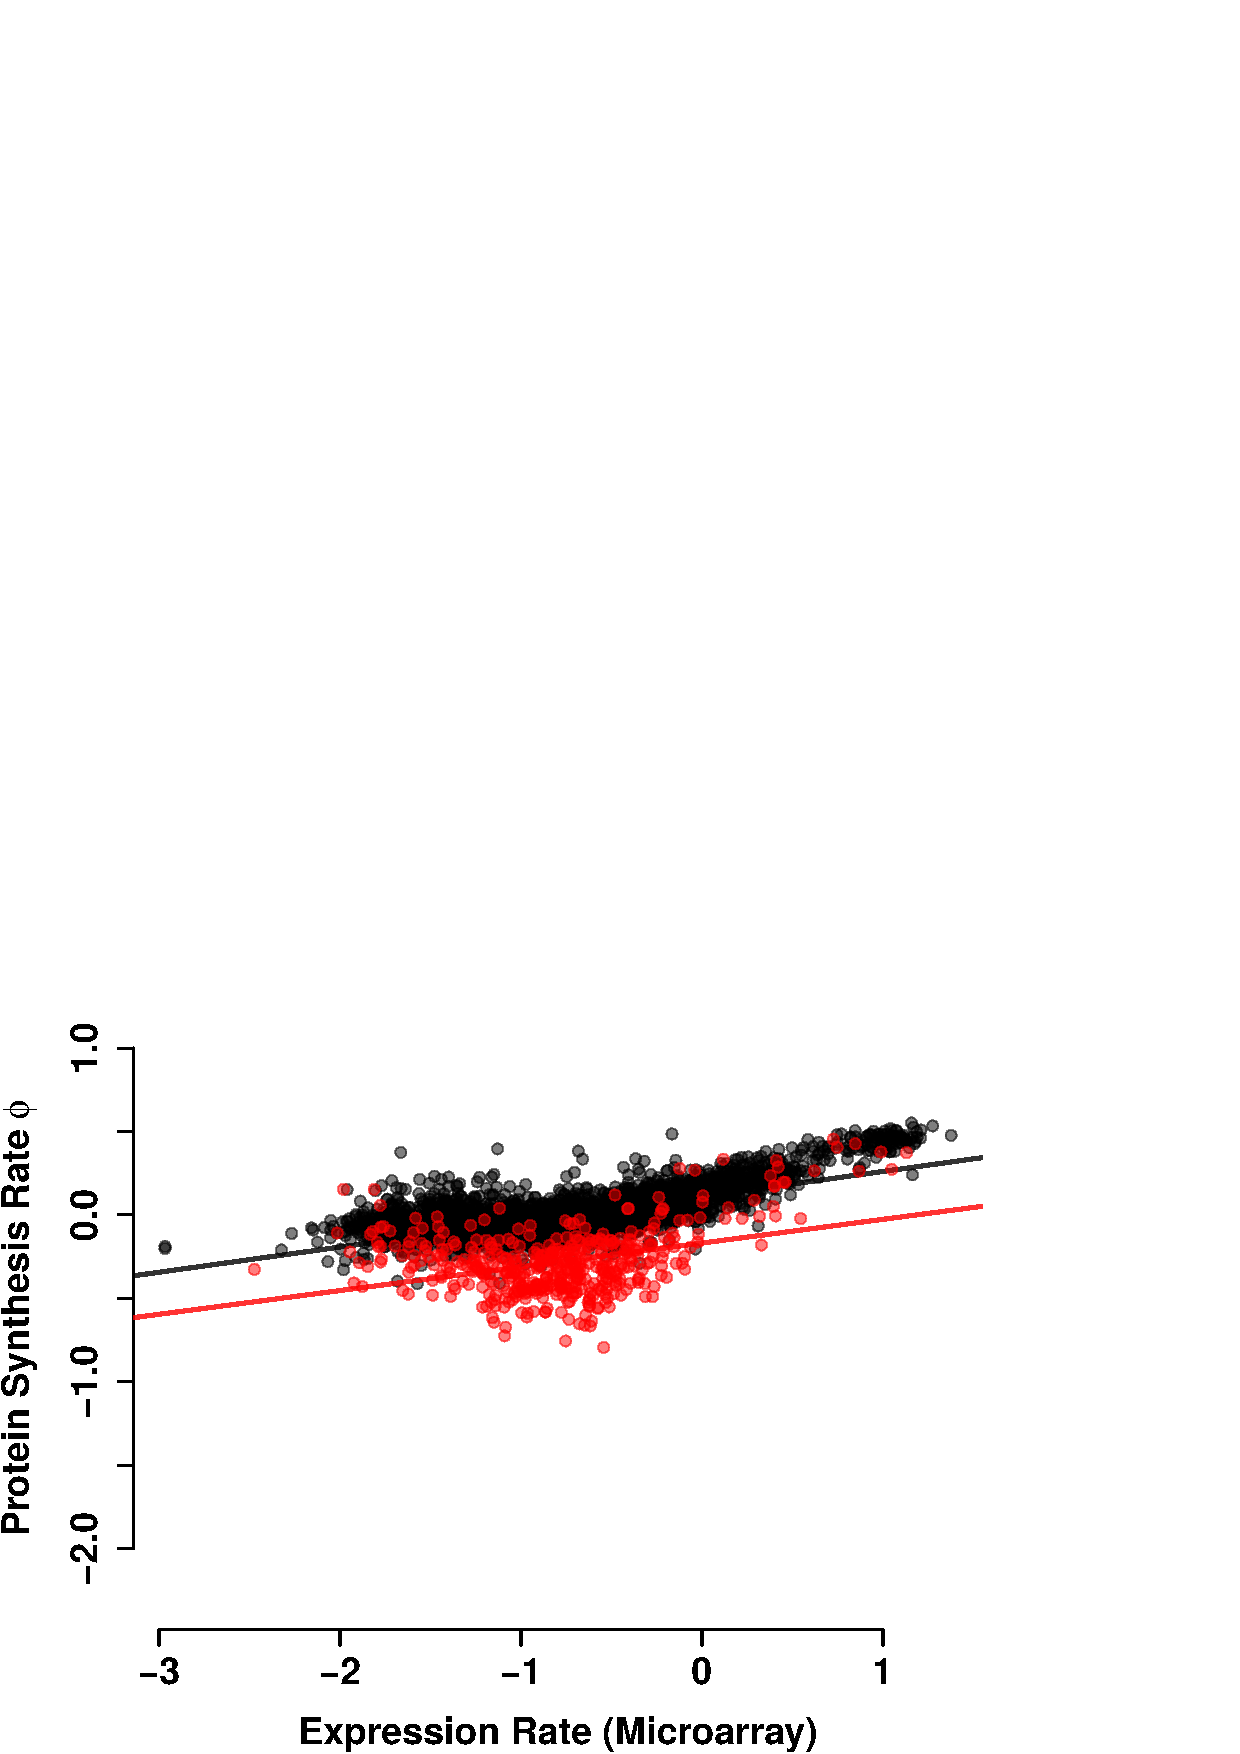
\includegraphics[width=.45\textwidth]{img/phi_corr_plot_whole_Genome_estim.pdf}
    \end{subfigure}
    \begin{subfigure}
        \centering
        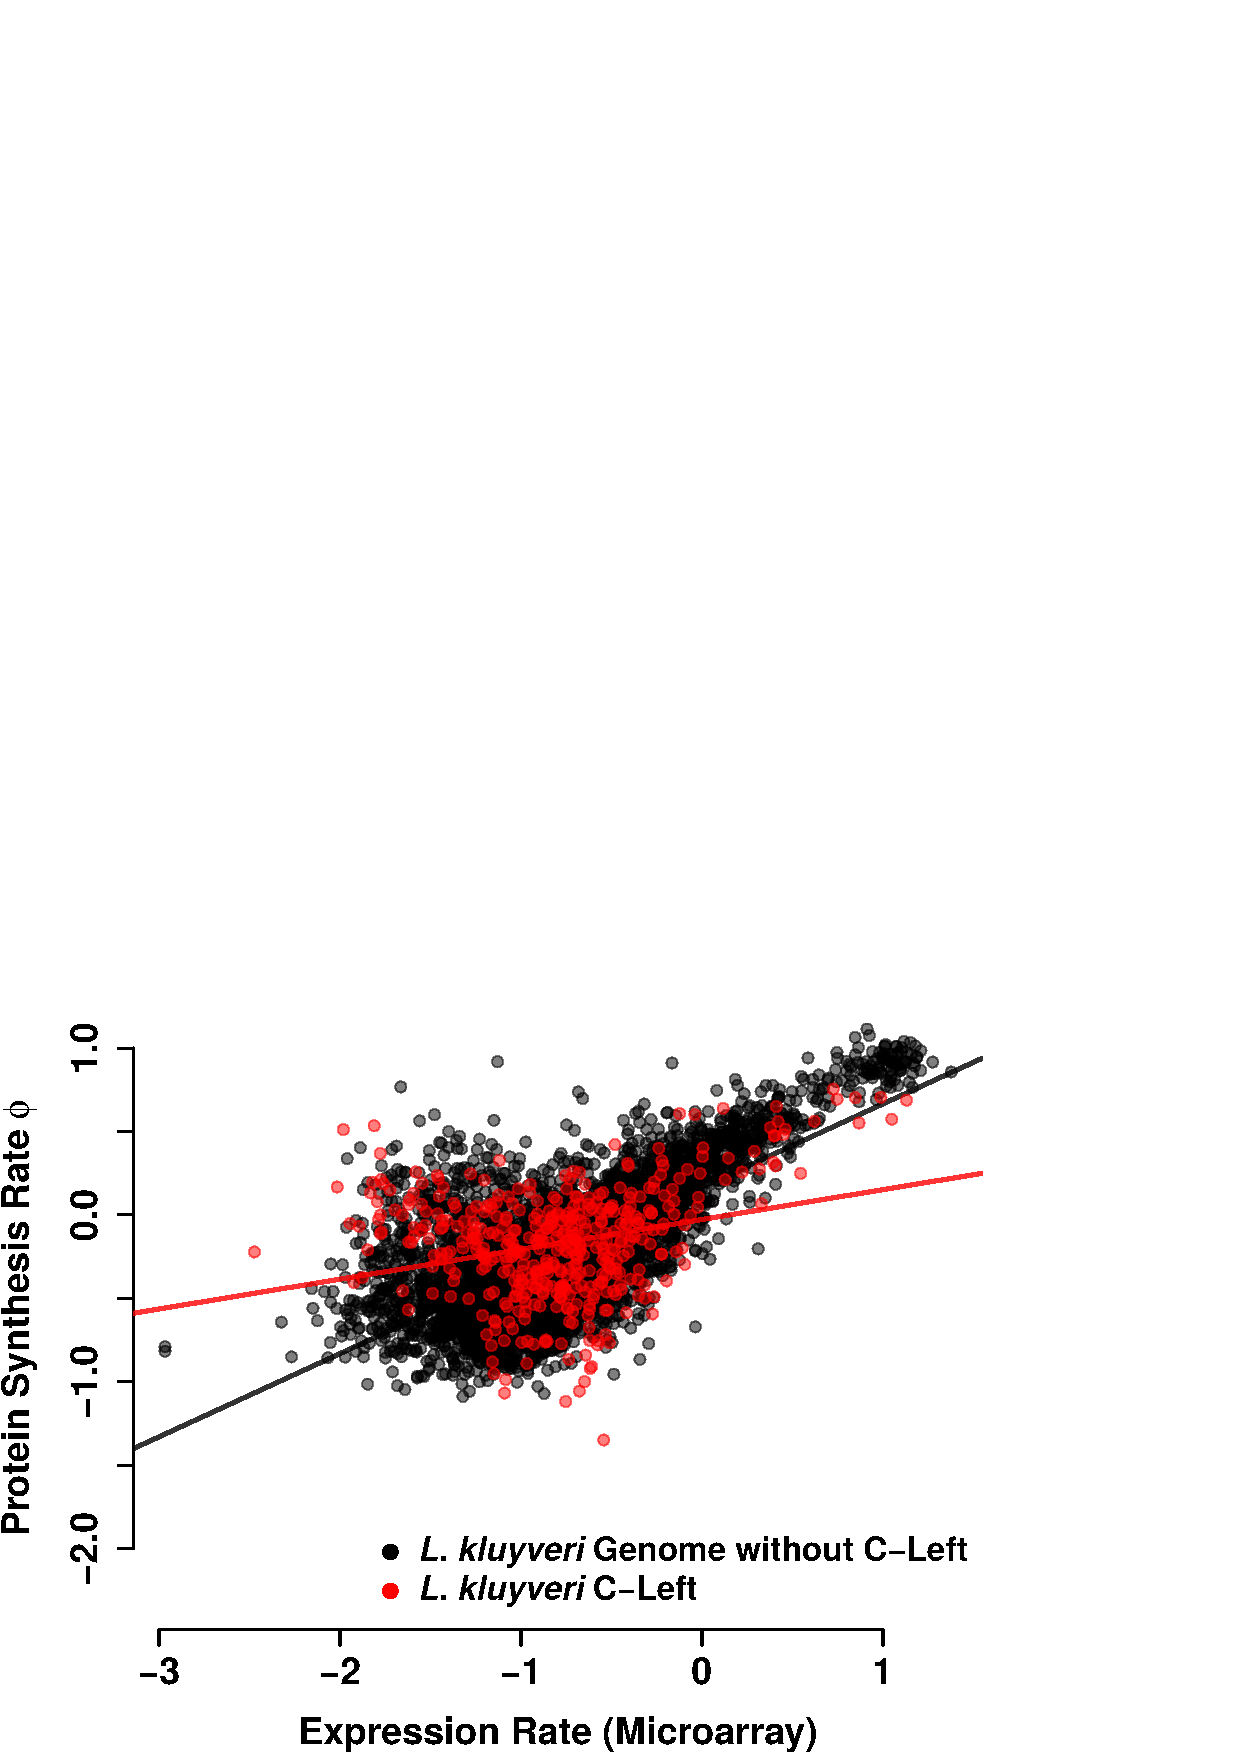
\includegraphics[width=.45\textwidth]{img/phi_corr_plot_split_Genome_estim.pdf}
    \end{subfigure}
    \caption{}
    \label{fig:phi_corr_two_cond}
\end{figure}


\begin{figure}[h]
    \centering
    \begin{subfigure}
        \centering
        \includegraphics[width=.45\textwidth]{img/csp_mean_correlation_endo.pdf}
    \end{subfigure}
    \begin{subfigure}
        \centering
        \includegraphics[width=.45\textwidth]{img/csp_mean_correlation_exo.pdf}
    \end{subfigure}
    \caption{}
    \label{fig:csp_endo_exo_comp}
\end{figure}


\begin{figure}[h]
    \centering
    \begin{subfigure}
        \centering
        \includegraphics[width=.45\textwidth]{img/fitness_difference_gos_kappa5.pdf}
    \end{subfigure}
    \begin{subfigure}
        \centering
        \includegraphics[width=.45\textwidth]{img/fitness_difference_exo.pdf}
    \end{subfigure}
    \caption{Fitness burden at time of introgression (left) using scaled $\phi$, and currently (right). }
    \label{fig:sne_fitness_burden}
\end{figure}

\clearpage
\section*{Suppl Figures}

\begin{figure}[h]
    \centering
    \begin{subfigure}
        \centering
        \includegraphics[width=.45\textwidth]{img/synteny_blocks_and_gc.pdf}
    \end{subfigure}
    \begin{subfigure}
        \centering
        \includegraphics[width=.45\textwidth]{img/synteny_coverage.pdf}
    \end{subfigure}
    \caption{Suppl Fig: Synteny relationship of \gossypii and the exogenous genes (left), Amount of synteny for each species (Units of std dev) checked for synteny.}
    \label{fig:synteny_species}
\end{figure}


\begin{figure}[h]
    \centering
    \begin{subfigure}
        \centering
        \includegraphics[width=.45\textwidth]{img/fitness_difference_gos_kappa1.pdf}
    \end{subfigure}
    \begin{subfigure}
        \centering
        \includegraphics[width=.45\textwidth]{img/fitness_phi_scaling_gos.pdf}
    \end{subfigure}
    \caption{Suppl Fig: Fitness burden (left) without scaling of $\phi$, and change of total fitness burden with scaling $\kappa$}
    \label{fig:sne_scaling}
\end{figure}

\clearpage
\begin{figure}[H]
     \centering
	\includegraphics[width=\textwidth]{img/CUB_cleft_main.pdf}
	\caption{Suppl Fig}
	\label{fig:corr_all_species}
\end{figure}

\end{document}